\chapter{Next-generation Non-volatile Memory Technology}
\label{sec:technology}

Research work on next-generation non-volatile memory technology has grown rapidly in recent years.
Worldwide research and development effort have been made on the emerging new memory devices \cite{wong2010phase}.
Before we move on to what we have done for the new design, we need to be clear about what exactly this
emerging new memory technology is. In this chapter, we will review the technical specifications
about the PCM technology. Besides, we will also talk about the challenges we face to design algorithms
for such systems and further our design considerations and targets.

\section{NVM Technology}

There are some widely pursued NVM technologies:
magneto-resistive random access memory (MRAM),
ferroelectric random access memories (FeRAM),
resistive random access memory (RRAM),
spin-transfer torque memory (STT-RAM),
and phase change memory (PCM).
As they have relatively similar features, in this work we focus on PCM since
it is at a more advanced stage of development and it can be expected to come out earlier.

Generally, NVM technologies share some features in common. Most NVM chips have comparable read latency than DRAM and rather
higher write latency. They have lower energy consumption but have limited endurance. Next we will review the technology details
of PCM technology. The physical technology of other NVMs may be different, but in this work, this is not our major focus and
we will mainly discuss about the PCM technology.
Since they share some of the common features, our design for PCM can be reused for other NVMs.

%PCM is a non-volatile memory that exploits the property of chalcogenide
%glass to switch between two states,
%amorphous and crystalline.
%The amorphous phase tends to have
%a high electrical resistivity,
%while the crystalline phase exhibits a low resistivity,
%giving rise to the so-called phase change materials.
%The two different phases can be switched
%%%: hww:start
%back-and-forth reliably and quickly.
%%%: hww:end
%For a large number of times,
%the difference in resistivity is typically about
%five orders of magnitude~\cite{raoux2008phase},
%which can be used to represent the two logical states of binary data.


\begin{figure}[!t]
\centering
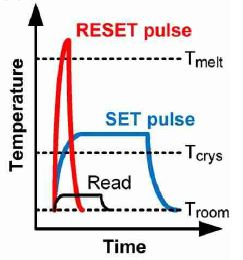
\includegraphics[scale=0.8]{figs/pcm.jpg}
\caption{PCM Technology}
\label{fig:pcm}
\end{figure}

PCM is a non-volatile memory that exploits the property of some phase change materials. The phase change material is one type of chalcogenide glass, such as $Ge_{2}Sb_{2}Te_{5}$ (GST) and it can be switched between two states, amorphous and crystalline by the current injection and the heating element. For a large number of times, the difference in resistivity is typically about five orders of magnitude~\cite{raoux2008phase}, which can be used to represent the two logical states of binary data. As we can see in Figure~\ref{fig:pcm}\cite{wong2010phase}, crystallizing the phase change material by heating it above the crystallization temperature ($\sim300^{\circ}$C) but below the melting temperature ($\sim600^{\circ}$C) is called the SET operation. The SET operation will turn GST into the crystalline state which corresponds to the logic `1'. Then when continuously heated above the melting temperature, GST turns into the amorphous state corresponding to the logic `0', which is called the RESET operation. Writes on phase change material will come down to the states switch, which incurs high operating temperature and further more latency and energy consumption. However, reads on phase change material just need to keep a much lower temperature, which can be faster and more energy saving.



%The phase change material is one type of alloy, such as $Ge_{2}Sb_{2}Te_{5}$ (GST) and the state switch of phase change materials is induced by the current injection and the heating element. Crystallizing the phase change material by heating it above the crystallization temperature ($\sim300^{\circ}$C) but below the melting temperature ($\sim600^{\circ}$C) is called the SET operation. The SET operation will turn GST into the crystalline state which corresponds to the logic `1'. Then when continuously heated above the melting temperature, GST turns into the amorphous state corresponding to the logic `0', which is called the RESET operation. Writes on phase change material will come down to the states switch, which incurs high operating temperature and further more latency and energy consumption. However, reads on phase change material just need to keep a much lower temperature, which can be faster and more energy saving.

We present a brief comparison on the properties
between PCM and other layers in the memory hierarchy,
including DRAM, NAND Flash (Solid State Drives, NAND for abbreviation)
and HDD (Hard Disk Drives).
Table \ref{tab:comparison} summarizes
the properties of these different memory technologies, as presented in recent
work \cite{chen2011rethinking, qureshi2009scalable, bedeschi2008multi} and the data all corresponds to raw memory chips.

\begin{table}\vspace*{-1em}
\centering \caption{Comparison of Memory Technologies}
\hspace*{-1em}\begin{tabular}{|c|c|c|c|c|} \hline
&DRAM&PCM&NAND&HDD \\ \hline \hline
Density&1X&2-4X&4X&N/A  \\ \hline
Read Latency&20-50ns&$\sim50ns$&$\sim25\mu s$&$\sim5ms$  \\
Write Latency&20-50ns&$\sim1\mu s$&$\sim500\mu s$&$\sim5ms$  \\ \hline
Read Energy&0.8J/GB&1J/GB&1.5J/GB&65J/GB  \\
Write Energy&1.2J/GB&6J/GB&17.5J/GB&65J/GB  \\ \hline
Endurance&$\infty$&$10^6-10^8$&$10^5-10^6$&$\infty$  \\ \hline
\end{tabular}
\label{tab:comparison}
\end{table}

From Table~\ref{tab:comparison},
we can see that the PCM has promising characteristics.
Compared to DRAM,
PCM has a density advantage over DRAM which means more memory capacity within
a same size chip and further a lower price per capacity.
This cheaper price can lead to orders of magnitude of capacity larger within the same budget.
Then the read and write performance is also very efficient. We can see that the read latency of PCM
is comparable to that of the DRAM.
Although writes are almost an order of magnitude slower than that of DRAM,
some techniques like buffer organization or partial writes could be used in
algorithms design to reduce the performance gap.
For NAND, the write on NAND should be based on pages and even though only
small parts of a page are modified, the whole page need to be rewritten, which is called the erase-before-writes problem.
NAND suffers from the erase-before-writes problem greatly and this issue caused the slow read and write speed
directly compared to DRAM and PCM.
Unlike NAND, PCM uses a totally different technology and it does not have the problem of erase-before-writes and
thus supports random reads and writes more efficiently.
We can see that reads and writes on PCM are
orders of magnitude faster than those of NAND and the endurance is also higher than that of NAND.
In summary, in most aspects, PCM can be seen as a technology in the middle between DRAM and NAND Flash.
Even though PCM has its own shortcomings but we believe that it will have a major role to play
in the memory hierarchy, impacting system performance, energy consumption and reliability because of its promising features.

\section{Positions in the Memory Hierarchy}

In previous section, we talked about the technical specifications of the 
PCM technology and we did a comparison between the several commonly used memory technologies. Now in this section, we want to talk about how to best integrate PCM into the existing memory systems, in other words, what is the proper position of PCM in the current memory hierarchy. 

\begin{figure}[!t]
\centering
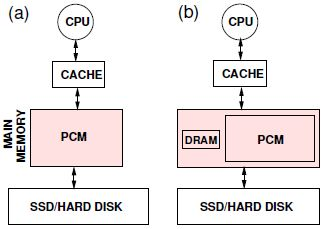
\includegraphics[scale=0.9]{figs/pcm-positions.jpg}
\caption{PCM Usage Proposals}
\label{fig:pcm-positions}
\end{figure}

In recent years, the computer systems community has already got various research proposals on how to make use of PCM technology in the current memory systems. Among all of them, 
there are mainly two schools of
thought~\cite{lee2009architecting,qureshi2009scalable,chen2011rethinking} as shown in Figure~\ref{fig:pcm-positions}\cite{chen2011rethinking}.
One is to replace DRAM with PCM directly
to achieve larger main memory capacity~\cite{lee2009architecting}.
Even though PCM is slower than DRAM,
Lee et al.~\cite{lee2009architecting} have shown that some
optimizations like buffer organization and partial writes can be
used to improve the system performance while preserving the
high density and non-volatile property.
The other proposal is
to replace the DRAM with a large PCM and a small
DRAM (3\% - 8\% size of the PCM
capacity \cite{qureshi2009scalable,ramos2011page}) and use
the DRAM as a buffer to keep some frequently
accessed data to improve the system performance.  
In this work, we will adopt the second approach, with the
use of PCM as ``extended'' but slower main memory and we will use a small number of DRAM as a buffer.



\section{Challenges to Algorithms Design}

Now we are clear about the features of PCM. Then before we start to design algorithms, we need to know the major challenges we face and the major target we want to reach. 

From the technologies comparison in previous sections, we can find the following three challenges we need to overcome. 

\begin{enumerate}
  \item Slow writes. Even the read and write speed is much faster than that of the NAND, it is still a bit slower than DRAM which will influence the system efficiency greatly.
      This challenge is the major one we want to overcome in this thesis. The idea is a bit trivial that since the writes are slow, we want to avoid writes as many as possible. 
  \item High energy consumption. This challenge is related to the writes. We know that each time we want to write values to the PCM chip, we need to switch its state. Then we need to heat to switch the state of the phase change material which leads to high energy consumption. But for read, since we do not need to switch the state, the energy consumption is much lower. 
  \item Limited endurance. Existing PCM prototypes have a write endurance ranging from $10^6$ to $10^8$ writes per cell \cite{chen2011rethinking}. With some good round robin or write leveling algorithms, a PCM main memory can last several years working time \cite{qureshi2009enhancing}. However, such kinds of algorithms should be conducted in the memory driver layer, which is not our main focus then. 
\end{enumerate}

From these challenges, we can find that actually if we want to make best use of PCM technology in our existing systems, the most important requirement is to figure out the challenge of high write latency. Our basic idea is that since the speed can not be raised physically, can we just avoid the writes as many as possible? 

Then The design objective becomes how to reduce the number of writes in our new algorithms which is an widely studied topic, especially the algorithms designed for NAND in recent years. However, our consideration
is different from that of the algorithms design for NAND. For NAND, they want to avoid the erase-before-writes and thus
they will mostly use the batch algorithms to convert random accesses to sequential writes. Our design consideration is different that
we can support random writes efficiently but we want to reduce the number of writes including both random writes and sequential
write as many as possible. Once the number of writes is limited, we can reduce the energy consumption and extend the life time as well. 


\section{Algorithms Design Considerations}

Let us go back to our initial problem that we want to make best use of PCM in the existing database systems and we want to integrate PCM into the memory systems. Thus we considering the algorithms design, we need to be careful about the following design goals: (1) CPU time, (2) CPU cache performance and (3) energy consumption. Compared to DRAM, the major shortcoming of PCM is the high write latency. Then for general algorithms, the slow write speed should not influence the cache performance, it can only influence the CPU execution time and energy consumption performance. We also know that the PCM writes incur much higher energy consumption and is much slower than read. Then the major challenge we are facing now is how to reduce the number of writes as many as possible. Actually we have already had this basic direction in mind in previous sections. 

Next the problem comes. We need a matric to measure the number of writes on the database algorithms level. In other words, we need to determine what granularity of writes we need to use in the algorithms analysis using PCM as the main memory. Generally when analyzing algorithms for main memory, we need to consider two granularities including bits and cache lines. For the high level database systems, we have the buffer management and it is easier to count the number of cache line based writes. However, in order to simulate the energy consumption, we need to get the number of writes based on the bits granularity.

Then we can use a mixture of these two metrics. To evaluate the CPU time, we count the number of writes based on the cache line granularity and to evaluate the energy consumption, we first compare the new cache line to the old cache line to get the number of modified bits and get the energy consumption then based on the bits level. Since we have not got any PCM prototype, we need to build a simulated environment to evaluate our algorithms. These should be configured in our simulated environment. 


\section{Summary}
In this chapter, we introduced the next-generation non-volatile memory technology. There are many kinds of popular non-volatile memory technologies and in this work, we will mainly focus on the phase change memory (PCM), but our algorithms can also be adaptive to other non-volatile memories having the similar features. We present the technical specification details of PCM and did a comparison among PCM and some commonly used memory technologies like DRAM, NAND and HDD about the major features. We found that PCM has its advantages, but there are also some challenges we need to overcome when designing algorithms for PCM-based database systems. Our main design goal is to avoid the slow writes as many as possible, which further can reduce the energy consumption and extend the lifetime of PCM chips. Finally, we discussed about some metrics to evaluate our new algorithms.

\newpage
%
